
\de{ĐỀ THI GIỮA HỌC KỲ I NĂM HỌC 2023-2024}{THPT LÊ TRỌNG TẤN }
\begin{center}
	\textbf{PHẦN 1 - TRẮC NGHIỆM}
\end{center}
\Opensolutionfile{ans}[ans/ans]

\begin{ex}%[0D1N1-4]%[Dự án đề kiểm tra Toán 10 GHKI NH23-24- Quang Anh]%[THPT Lê Trọng Tấn]
	Mệnh đề đảo của mệnh đề $P\Rightarrow Q$ là mệnh đề nào?
	\choice{\True $Q\Rightarrow P$}
	{$Q\Rightarrow\overline{P}$}
	{$Q\Rightarrow\overline{P}$}
	{$\overline{Q} \Rightarrow P$}
	\loigiai{
		Mệnh đề đảo của mệnh đề $P\Rightarrow Q$ là mệnh đề $Q\Rightarrow P$.
	}
\end{ex}

\begin{ex}%[0D1N1-1]%[Dự án đề kiểm tra Toán 10 GHKI NH23-24- Quang Anh]%[THPT Lê Trọng Tấn]
	Trong các câu sau, câu nào không phải là một mệnh đề
	\choice
	{\True Ăn phở rất ngon!}
	{Hà nội là thủ đô của Việt Nam}
	{Số $18$ chia hết cho $6$}
	{$2+8=6$}
	\loigiai{
		Ăn phở rất ngon! đây là câu cảm thán nên không phải là một mệnh đề.
	}
\end{ex}

\begin{ex}%%[0D1N3-3][Dự án đề kiểm tra Toán 10 GHKI NH23-24- Quang Anh]%[THPT Lê Trọng Tấn]
	Cho $A=\{x\in\mathbb{R}\mid x \leq-3\}, B=\{x \in \mathbb{R} \mid -3 < x \leq 10\}$. Khi đó $A\cup B$ bằng?
	\choice{$[-3; 10]$}
	{\True $(-\infty; 10]$}
	{$\{-3\}$}
	{$\varnothing$}
	\loigiai{
		Ta có $A\cup B =(-\infty; 10]$.
	}
\end{ex}

\begin{ex}%[0D1H3-5]%[Dự án đề kiểm tra Toán 10 GHKI NH23-24- Quang Anh]%[THPT Lê Trọng Tấn]
	Trong kì thi học sinh giỏi cấp trường, lớp $10 \mathrm{~A}$ có 15 học sinh thi học sinh giỏi môn Ngữ văn, $20$ học sinh thi học sinh giỏi môn Toán. Tìm số học sinh thi cả hai môn Ngữ văn và Toán. Biết lớp $10 \mathrm{~A}$ có $40$ học sinh và có $10$ học sinh không thi cả môn Toán và Ngữ văn.
	\choice
	{$6$}
	{\True $5$}
	{$4$}
	{$3$}
	\loigiai{
		Gọi $A$, $B$, $C$ lần lượt là tập hợp các học sinh thi học sinh giỏi cấp trường môn Toán, Văn và không thi cả môn Toán và Văn.\\
		Khi đó $n(A)=20$, $n(B)=15$, $n(C)=10$, $n(A\cup B\cup C)=40$.\\
		Mà $n(A\cup B\cup C)=n(A)+n(B)-n(A\cap B)+n(C)\Rightarrow n(A\cap B) =20+15-40+10=5$.\\
		Vậy lớp $10 \mathrm{~A}$ có số học sinh thi cả hai môn Ngữ văn và Toán là $5$ học sinh.
	}
\end{ex}

\begin{ex}%[0D2N1-1]%[Dự án đề kiểm tra Toán 10 GHKI NH23-24- Quang Anh]%[THPT Lê Trọng Tấn]
	Cặp số nào là một nghiêm của bất phương trình $2x+3y \leq 5$?
	\choice
	{$(1; 2)$}
	{\True $(-2; 1)$}
	{$(5; 3)$}
	{$(-1; 4)$}
	\loigiai{
		Ta thấy cặp số $(-2; 1)$ thỏa mãn bất phương trình $2x+3y \leq 5$. Do đó cặp số $(-2; 1)$ là một nghiêm của bất phương trình đã cho.
	}
\end{ex}

\begin{ex}%[0H4N1-1]%[Dự án đề kiểm tra Toán 10 GHKI NH23-24- Quang Anh]%[THPT Lê Trọng Tấn]
	Với giá trị nào của $\alpha$ thì $\cos \alpha > 0$?
	\choice
	{$0^{\circ} < \alpha \leq 90^{\circ}$}
	{$90^{\circ} < \alpha \leq 180^{\circ}$}
	{$0^{\circ} \leq \alpha \leq 90^{\circ}$}
	{\True $0^{\circ} \leq \alpha < 90^{\circ}$}
	\loigiai{
		Với $0^{\circ} \leq \alpha < 90^{\circ}$ thì $\cos \alpha > 0$.
	}
\end{ex}
%7
\begin{ex}%[0H4H2-1]%[Dự án đề kiểm tra Toán 10 GHKI NH23-24- Thehung Nguyen]%[THPT LÊ TRỌNG TÁN - Tp HCM]
	Tam giác $A B C$ có các cạnh $a=3 \sqrt{3}$ cm, $b=6$ cm, $c=3$ cm. Độ lớn của góc $A$ là
	\choice
	{$45^{\circ}$}
	{$120^{\circ}$}
	{\True $60^{\circ}$}
	{$30^{\circ}$}
	\loigiai{
		Áp dụng định lý hàm số cosin trong $\triangle ABC$ ta có\\
		$\cos A=\dfrac{b^2+c^2-a^2}{2bc}=\dfrac{36+9-27}{36}=\dfrac{1}{2}\Rightarrow A=60^\circ$.
	}
\end{ex}

%8
\begin{ex}%[0H4N2-2]%[Dự án đề kiểm tra Toán 10 GHKI NH23-24- Thehung Nguyen]%[THPT LÊ TRỌNG TÁN - Tp HCM]
	Chọn công thức đúng trong các đáp án sau
	\choice
	{\True $S=\dfrac{1}{2} b c \sin A$}
	{$S=\dfrac{1}{2} a c \sin A$}
	{$S=\dfrac{1}{2} b c \sin B$}
	{$S=\dfrac{1}{2} b c \sin C$}
	\loigiai{Diện tích tam giác theo công thức $S=\dfrac{1}{2} b c \sin A$.
	}
\end{ex}

%9
\begin{ex}%[0D1H2-2]%[Dự án đề kiểm tra Toán 10 GHKI NH23-24- Thehung Nguyen]%[THPT LÊ TRỌNG TÁN - Tp HCM]
	Cho $A=\{1 ; 2 ; x ; y, z\}$, số tập con của $A$ là
	\choice
	{$10$}
	{\True $32$}
	{$5$}
	{$16$}
	\loigiai{Số tập con của $A$ là $2^5=32$.
	}
\end{ex}

%10
\begin{ex}%[0D1N2-2]%[Dự án đề kiểm tra Toán 10 GHKI NH23-24- Thehung Nguyen]%[THPT LÊ TRỌNG TÁN - Tp HCM]
	Cho tập hợp $T=\{1,4,6\}$. Tập hợp nào sau đây là tập con của $T$?
	\choice
	{$T_3=\{0,4\}$}
	{\True $T_1=\varnothing$}
	{$T_2=\{2,7\}$}
	{$T_4=\{0\}$}
	\loigiai{Ta có $T_1=\varnothing$ là con của $T$.
	}
\end{ex}

%11
\begin{ex}%[0D2H1-2]%[Dự án đề kiểm tra Toán 10 GHKI NH23-24- Tacgia]%[THPT LÊ TRỌNG TÁN - Tp HCM]
	\immini{Chọn bất phương trình mà miền nghiệm của nó là nửa mặt phẳng không bị gạch có bờ là đường thẳng $\Delta$, kể cả bờ $\Delta$ như hình bên.		
		\choice
		{$2 x-y+4<0$}
		{ $2 x-y+4>0$}
		{\True$2 x-y+4 \leq 0$}
		{$x-2 y+4 \leq 0$}}{\begin{tikzpicture}[scale=0.9,line join=round, line cap=round,>=stealth,thick]
			%\tikzset{every node/.style={scale=0.9}}
			\begin{scope}
				\draw[->] (-3,0)--(2,0) node[below]{$x$};
				\draw[->] (0,-1)--(0,5) node[left]{$y$};
				\path 
				(-2,0)node[above left]{$-2$}
				(0,4)node[left]{$4$}
				;
				\clip (-2.5,-1) rectangle (1.95,5);
				\fill[pattern=north east lines] (-5,-6)--(3,-6)--(3,10)--cycle;
				\draw (0.5,5)--(-2.5,-1);
				
				\draw (0,0) node[below left]{$O$};
				
			\end{scope}	
	\end{tikzpicture}}	
	\loigiai{Vì miền nghiệm kể bờ của nó nên loại phương án $2 x-y+4 < 0$ và $x-2 y+4 > 0$.\\		
		Ta có $A(0;4)$ thuộc $ \Delta$ mà không thuộc $x-2 y+4$ vì $0-2\cdot 4+4\ne 0$ nên loại phương án $x-2 y+4 \leq 0$.\\
		Vậy phương án thỏa đề bài là $2 x-y+4 \leq 0$.
	}
\end{ex}

%12
\begin{ex}%[0H4H1-3]%[Dự án đề kiểm tra Toán 10 GHKI NH23-24- Thehung Nguyen]%[THPT LÊ TRỌNG TÁN - Tp HCM]
	Rút gọn biểu thức sau $A=(\tan x+\cot x)^2-(\tan x-\cot x)^2$.
	\choice
	{\True $A=4$}
	{$A=1$}
	{$A=2$}
	{$A=3$}
	\loigiai{Ta có 
		\begin{eqnarray*}
			A&=&(\tan x+\cot x)^2-(\tan x-\cot x)^2\\
			&=& \tan^2x+2\tan x\cot x+\cot^2x-\tan^x+2\tan x\cot x-cot^2x\\\
			&=& 2+2=4.
		\end{eqnarray*}
	}
\end{ex}



\Closesolutionfile{ans}
%\begin{center}
%	\textbf{ĐÁP ÁN}
%	\inputansbox{10}{ans/ans}	
%\end{center}
\begin{center}
	\textbf{PHẦN 2 - TỰ LUẬN}
\end{center}


%Câu 1...........................
\begin{bt}%[0D1H1-2]%[0D1H1-3]%[Dự án đề kiểm tra Toán 10 GHKI NH23-24- Đặng Tân Hoài]%[THPT LÊ TRỌNG TẤN - Tp Hồ Chí Minh]
	Xét tính đúng sai và viết mệnh đề phủ định của các mệnh đề sau:
	\begin{enumerate}
		\item \lq\lq $\forall x \in \mathbb{R}, ~x^2+2x+2>0$ \rq\rq.
		\item \lq\lq $\exists x \in \mathbb{R}, ~x^2+3x+4=0$ \rq\rq.
	\end{enumerate}
	\loigiai{
		\begin{enumerate}
			\item Mệnh đề đúng; vì bất kì $\forall x \in \mathbb{R}$, ta đều có $$x^2+2x+2=(x^2+2x+1)+1=(x+1)^2+1\ge 1 >0.$$
			Mệnh đệ phủ định của mệnh đề đã cho là
			\lq\lq $\exists x \in \mathbb{R}, ~x^2+2x+2\le 0$ \rq\rq.
			\item Mệnh đề sai; vì bất kì $\forall x \in \mathbb{R}$, ta đều có phương trình $x^2+3x+4=0$ vô nghiệm.\\
			Mệnh đệ phủ định của mệnh đề đã cho là
			\lq\lq $\forall x \in \mathbb{R}, ~x^2+3x+4\ne 0$ \rq\rq.
		\end{enumerate}
	}
\end{bt}

%Câu 2...........................
\begin{bt}%[0D1H2-1]%[Dự án đề kiểm tra Toán 10 GHKI NH23-24- Đặng Tân Hoài]%[THPT LÊ TRỌNG TẤN - Tp Hồ Chí Minh]
	Viết tập hợp sau đây dưới dạng liệt kê các phần tử và tìm số phần tử của mỗi tập hợp đó:
	\begin{enumerate}
		\item $A=\left\lbrace x\in \mathbb{R}\,\mid\, x^2-2x+3=0 \right\rbrace$.
		\item $B=\left\lbrace n\in \mathbb{N}\,\mid\, n \text{ là bội của }5 \text{ và } n\le 30 \right\rbrace$.
	\end{enumerate}
	\loigiai{
		\begin{enumerate}
			\item Vì phương trình $x^2-2x+3=0$ vô nghiệm nên $A=\varnothing$. Số phần tử của $A$ là $0$.
			\item Ta có $B=\left\lbrace 5;10;15;20;25;30\right\rbrace$, số phần tử của $B$ là $6$.
		\end{enumerate}			
	}
\end{bt}

%Câu 3...........................
\begin{bt}%[0D1H3-3]%[0D1H3-4]%[Dự án đề kiểm tra Toán 10 GHKI NH23-24- Đặng Tân Hoài]%[THPT LÊ TRỌNG TẤN - Tp Hồ Chí Minh]
	Cho hai tập hợp $A=(-3;5)$, $B=[2;7)$. Hãy tìm $A\cap B$, $\mathrm{C}_{\mathbb{R}} A$.
	\loigiai{
		Ta có 
		\begin{itemize}
			\item \immini{
				$A\cap B = [2;5)$
			}{\vspace*{-0.5cm}
				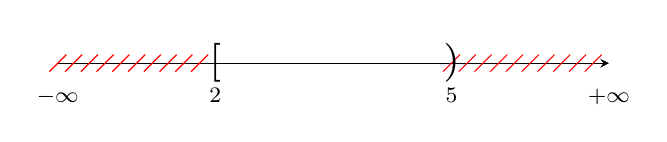
\begin{tikzpicture}[font=\footnotesize, line join=round, line cap=round, >=stealth]
					\tikzset{giao/.pic={
							\draw[->](0,0)--(7,0);
							\foreach \i in{0,0.2,...,1.8,5.0,5.2,...,6.8}
							\draw[red](\i,0)--++(45:0.15)(\i,0)--++(-135:0.15);
							\path(2,0)node[scale=1.75]{$[$}(5,0)node[scale=1.75]{$)$};
							\path(2,0)node[below=2mm]{$2$}(5,0)node[below=2mm]{$5$};
							\path(0,0)node[below=2mm]{$-\infty$}(7,0)node[below=2mm]{$+\infty$};
					}}
					\path (0,0)pic{giao};
			\end{tikzpicture}	}
			\item \immini{
				$\mathrm{C}_{\mathbb{R}} A = \mathbb{R}\setminus A = (-\infty;-3] \cup [5;+\infty)$
			}{\vspace*{-0.5cm}
				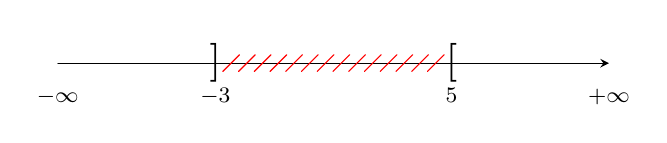
\begin{tikzpicture}[font=\footnotesize, line join=round, line cap=round, >=stealth]
					\tikzset{bu/.pic={
							\draw[->](0,0)--(7,0);
							\foreach \i in{2.2,2.4,...,4.8}
							\draw[red](\i,0)--++(45:0.15)(\i,0)--++(-135:0.15);
							\path(2,0)node[scale=1.75]{$]$}(5,0)node[scale=1.75]{$[$};
							\path(2,0)node[below=2mm]{$-3$}(5,0)node[below=2mm]{$5$};
							\path(0,0)node[below=2mm]{$-\infty$}(7,0)node[below=2mm]{$+\infty$};
					}}
					\path (0,0)pic{bu};
			\end{tikzpicture}	}
		\end{itemize}
	}
\end{bt}

%Câu 4...........................
\begin{bt}%[0D1V3-3]%[Dự án đề kiểm tra Toán 10 GHKI NH23-24- Đặng Tân Hoài]%[THPT LÊ TRỌNG TẤN - Tp Hồ Chí Minh]
	Cho hai tập hợp $A=(1;5)$, $B=(m;m+1)$. Tìm tham số $m$ để $A\cap B$ là một khoảng.
	\loigiai{
		Điều kiện tồn tại tập hợp $B$ là $m<m+1$, luôn đúng $\forall m \in \mathbb{R}$.\\
		Xét ngược yêu cầu bài toán, ta có
		$$A\cap B=\varnothing \Leftrightarrow \hoac{& m+1\le 1 \\& m\ge 5} \Leftrightarrow \hoac{& m\le 0\\& m\ge 5 .}$$
		Vậy $A\cap B$ là một khoảng khi $0<m<5$.
	}
\end{bt}

%Câu 5...........................
\begin{bt}%[0D2H1-2]%[Dự án đề kiểm tra Toán 10 GHKI NH23-24- Đỗ Đường Hiếu]%[THPT LÊ TRỌNG TẤN - Tp Hồ Chí Minh]
	Biểu diễn miền nghiệm của bất phương trình $5x-7y\le 0$ trên mặt phẳng tọa độ.
	\loigiai{
	Vẽ đường thẳng $d\colon 5x-7y=0$.\\
	Xét điểm $A(-1;0)$, ta có $5\cdot 1-7\cdot 0=5>0$. Suy ra miền nghiệm của bất phương trình $5x-7y\le 0$ là nửa mặt phẳng bờ $d$ chứa điểm $A$.
	\begin{center}
		\begin{tikzpicture}[scale=0.8,font=\footnotesize, line join=round, line cap=round, >=stealth]
			\draw[->] (-3,0)--(3,0) node[below]{$x$};
			\draw[->] (0,-2)--(0,2.5) node[right]{$y$};
			\begin{scope}
				\clip (-3,-2) rectangle (3,2.5);
				\draw plot[smooth,domain=-3:3] (\x,{(5/7)*(\x)});
				\fill [pattern=north east lines] (-7,-5)--(3,-2)--(7,5)--cycle;
			\end{scope}
			\path 
			(0,0) node[below right]{$O$}
			(-1,0) node[above]{$-1$};
			\fill[black] (0,0) circle(1.4 pt) (-1,0) circle(1.4 pt);
		\end{tikzpicture}
	\end{center}
	}
\end{bt}

%Câu 6...........................
\begin{bt}%[0D2V2-3]%[Dự án đề kiểm tra Toán 10 GHKI NH23-24- Đỗ Đường Hiếu]%[THPT LÊ TRỌNG TẤN - Tp Hồ Chí Minh]
	Gia đình cần ít nhất $900$ đơn vị protein và $400$ đơn vị lipit trong thức ăn mỗi ngày. Mỗi kilogam thịt bò chứa 800 đơn vị protein và $200$ đơn vị lipit. Mỗi kilogam thịt lợn chứa $600$ đơn vị protein và $400$ đơn vị lipit. Biết rằng mỗi ngày gia đình này chỉ mua tối đa $1{,}5$ kg thịt bò và $1$ kg thịt lợn, giá tiền $1$ kg thịt bò là $200$ nghìn đồng, $1$ kg thịt lợn là $100$ nghìn đồng. Hỏi gia đình đó phải mua bao nhiêu kg thịt mỗi loại để số tiền bỏ ra là ít nhất?
	\loigiai{
	Gọi $x$, $y$ lần lượt là số kg thịt bò, thịt lợn gia đình mua ($0\le x\le 1{,}5$, $0\le y\le 1$).\\
	Khi đó ta có hệ bất phương trình
	$$\heva{&800x+600y\ge 900\\&200x+400y\ge 400\\&0\le x\le 1{,}5\\& 0\le y\le 1}\Leftrightarrow \heva{&8x+6y\ge 9\\&x+2y\ge 2\\&0\le x\le 1{,}5\\&0\le y\le 1.}\qquad (*)$$
	Chi phí gia đình bỏ ra để mua thịt là $F(x;y)=200x+100y$ (nghìn đồng).\\
	Miền nghiệm của hệ $(*)$ là miền tứ giác $ABCD$, với $A(1{,}5;0{,}25)$, $B(1{,}5;1)$, $C\left(\dfrac{3}{8};1\right)$ và $D\left(\dfrac{3}{5};\dfrac{7}{10}\right)$.\\
	Giá trị lớn nhất hay nhỏ nhất của $F(x;y)$ với $(x;y)$ là nghiệm của hệ $(*)$ đạt được tại một trong các đỉnh $A$, $B$, $C$, $D$.
	\begin{itemize}
		\item Tại $A(1{,}5;0{,}25)$, ta có $F=325$.
		\item Tại $B(1{,}5;1)$, ta có $F=400$.
		\item Tại $C\left(\dfrac{3}{8};1\right)$, ta có $F=175$.
		\item Tại $D\left(\dfrac{3}{5};\dfrac{7}{10}\right)$, ta có $F=190$.
	\end{itemize}
	Vậy, để số tiền bỏ ra ít nhất thì gia đình đó mua $\dfrac{3}{8}$ kg thịt bò và $1$ kg thịt lợn.
	\begin{center}
		\begin{tikzpicture}[scale=2,font=\footnotesize, line join=round, line cap=round, >=stealth]
			\draw[->] (-0.5,0)--(2.6,0) node[below]{$x$};
			\draw[->] (0,-0.5)--(0,2.1) node[right]{$y$};
			\begin{scope}
				\clip (-.5,-.5) rectangle (2.5,2);
				\draw plot[smooth,domain=-1:2] (\x,{(-4/3)*(\x)+(3/2)});
				\fill [pattern=north east lines] (-3,5.5)--(-0.5,-0.5)--(3,-2.5)--cycle;
				\draw plot[smooth,domain=-1:2.5] (\x,{-0.5*(\x)+1});
				\fill [pattern=north east lines] (-1,1.5)--(-1,-1)--(3,-0.5)--cycle;
				\fill [pattern=horizontal lines] (1.5,-0.5)--(1.5,2)--(2.5,2)--(2.5,-0.5)--cycle;
				\fill [pattern=horizontal lines] (-0.5,-0.5)--(-0.5,2)--(0,2)--(0,-0.5)--cycle;
				\fill [pattern=vertical lines] (-0.5,-0.5)--(-0.5,0)--(2,0)--(2,-0.5)--cycle;
				\fill [pattern=vertical lines] (-0.5,1)--(2.5,1)--(2.5,2)--(-0.5,2)--cycle;
				\draw (1.5,-0.5)--(1.5,2) (-0.5,1)--(2.5,1) ;
			\end{scope}
			\path 
			(0,0) node[below right]{$O$}
			(1.5,0) node[above left]{$1{,}5$}
			(1.5,0.25) node[above right]{$A$}
			(1.5,1) node[below right]{$B$}
			(0.375,1) node[above right]{$C$}
			(0.6,0.7) node[above right]{$D$}
			(0,1) node[left]{$1$};
			\fill[black] (0,0) circle(0.7 pt) (1.5,0) circle(1 pt) (0,1) circle(0.7 pt)  (1.5,0.25) circle(0.7 pt)  (0.375,1) circle(0.7 pt)  (1.5,1) circle(0.7 pt)  (0.6,0.7) circle(0.7 pt) ;
		\end{tikzpicture}
	\end{center}
	}
\end{bt}%[0D2V2-3]}

%Câu 7...........................
\begin{bt}%[0H4H1-2]%[Dự án đề kiểm tra Toán 10 GHKI NH23-24- Đỗ Đường Hiếu]%[THPT LÊ TRỌNG TẤN - Tp Hồ Chí Minh]
	Cho $\cos\alpha= -\dfrac{1}{2}$ và $90^\circ<\alpha<180^\circ$. Tính $\sin \alpha$ và $\cot \alpha$.
	\loigiai{
	Ta có
	\begin{itemize}
		\item Vì $90^\circ<\alpha<180^\circ$ nên $\sin\alpha >0$. Do đó
		$$\sin\alpha=\sqrt{1-\cos^2\alpha}=\sqrt{1-\left(-\dfrac{1}{2}\right)^2}=\dfrac{\sqrt{3}}{2}.$$
		\item $\cot \alpha=\dfrac{\cos \alpha}{\sin\alpha}= -\dfrac{1}{2}:\dfrac{\sqrt{3}}{2}=\dfrac{\sqrt{3}}{3}$.
	\end{itemize}
	}
\end{bt}

%Câu 8...........................
\begin{bt}%[0H4V2-2]%[Dự án đề kiểm tra Toán 10 GHKI NH23-24- Đỗ Đường Hiếu]%[THPT ]
	\immini{Cho tam giác $ABC$ có $AB=4$, $BC=6$, $\widehat{ABC}=120^\circ$ (tham khảo hình vẽ). Tính độ dài cạnh $AC$ và độ dài đường cao $BH$ của tham giác $ABC$.}
	{\begin{tikzpicture}[scale=1, line cap=round,line join=round,font=\footnotesize]
			\path
			(0:0) coordinate (A)
			(0:4) coordinate (C)
			(46.5:2) coordinate (B)
			($(A)!(B)!(C)$) coordinate (H)
			;
			\draw (A)--(B)--(C)--cycle (B)--(H)
			;
			\pic [draw, angle eccentricity=1.5] {angle = A--B--C};
			\foreach \x/\g in {A/180,B/90,C/0,H/-90} \draw[fill=black] (\x) circle (.05) +(\g:.3) node {$\x$}
			;
	\end{tikzpicture}
}
	\loigiai{
	\begin{itemize}
		\item $AC^2=AB^2+BC^2-2\cdot AB\cdot BC \cos \widehat{ABC}=4^2+6^2-2\cdot 4\cdot 6\cdot \cos 120^\circ=76$.\\
		Suy ra $AC=2\sqrt{19}$.
		\item $S_{\triangle ABC}=\dfrac{1}{2}AB\cdot BC\cdot\sin \widehat{ABC}=120^\circ=\dfrac{1}{2}\cdot 4\cdot 6\cdot \sin 120^\circ=6\sqrt{3}$.\\
		Do đó, độ dài đường cao $BH$ là $BH=\dfrac{2S_{\triangle ABC}}{AC}=\dfrac{2\cdot 6\sqrt{3}}{2\sqrt{19}}=\dfrac{6\sqrt{57}}{19}$.
	\end{itemize}
	}
\end{bt}
